\chapter{Felhasználói dokumentáció}
\label{ch:user}

\section{Áttekintés}

Az alkalmazás böngészőben fut. Egy oldalból áll, mely nagy részét egy interaktív térkép foglalja el (\ref{fig:screenshot-welcome}). A képernyő bal oldalán egy vezérlőpanel található, melyen keresztül az alkalmazás irányítható. Az alkalmazás használatához nincs szükség regisztrációra vagy bejelentkezésre.

\begin{figure}[H]
	\centering
	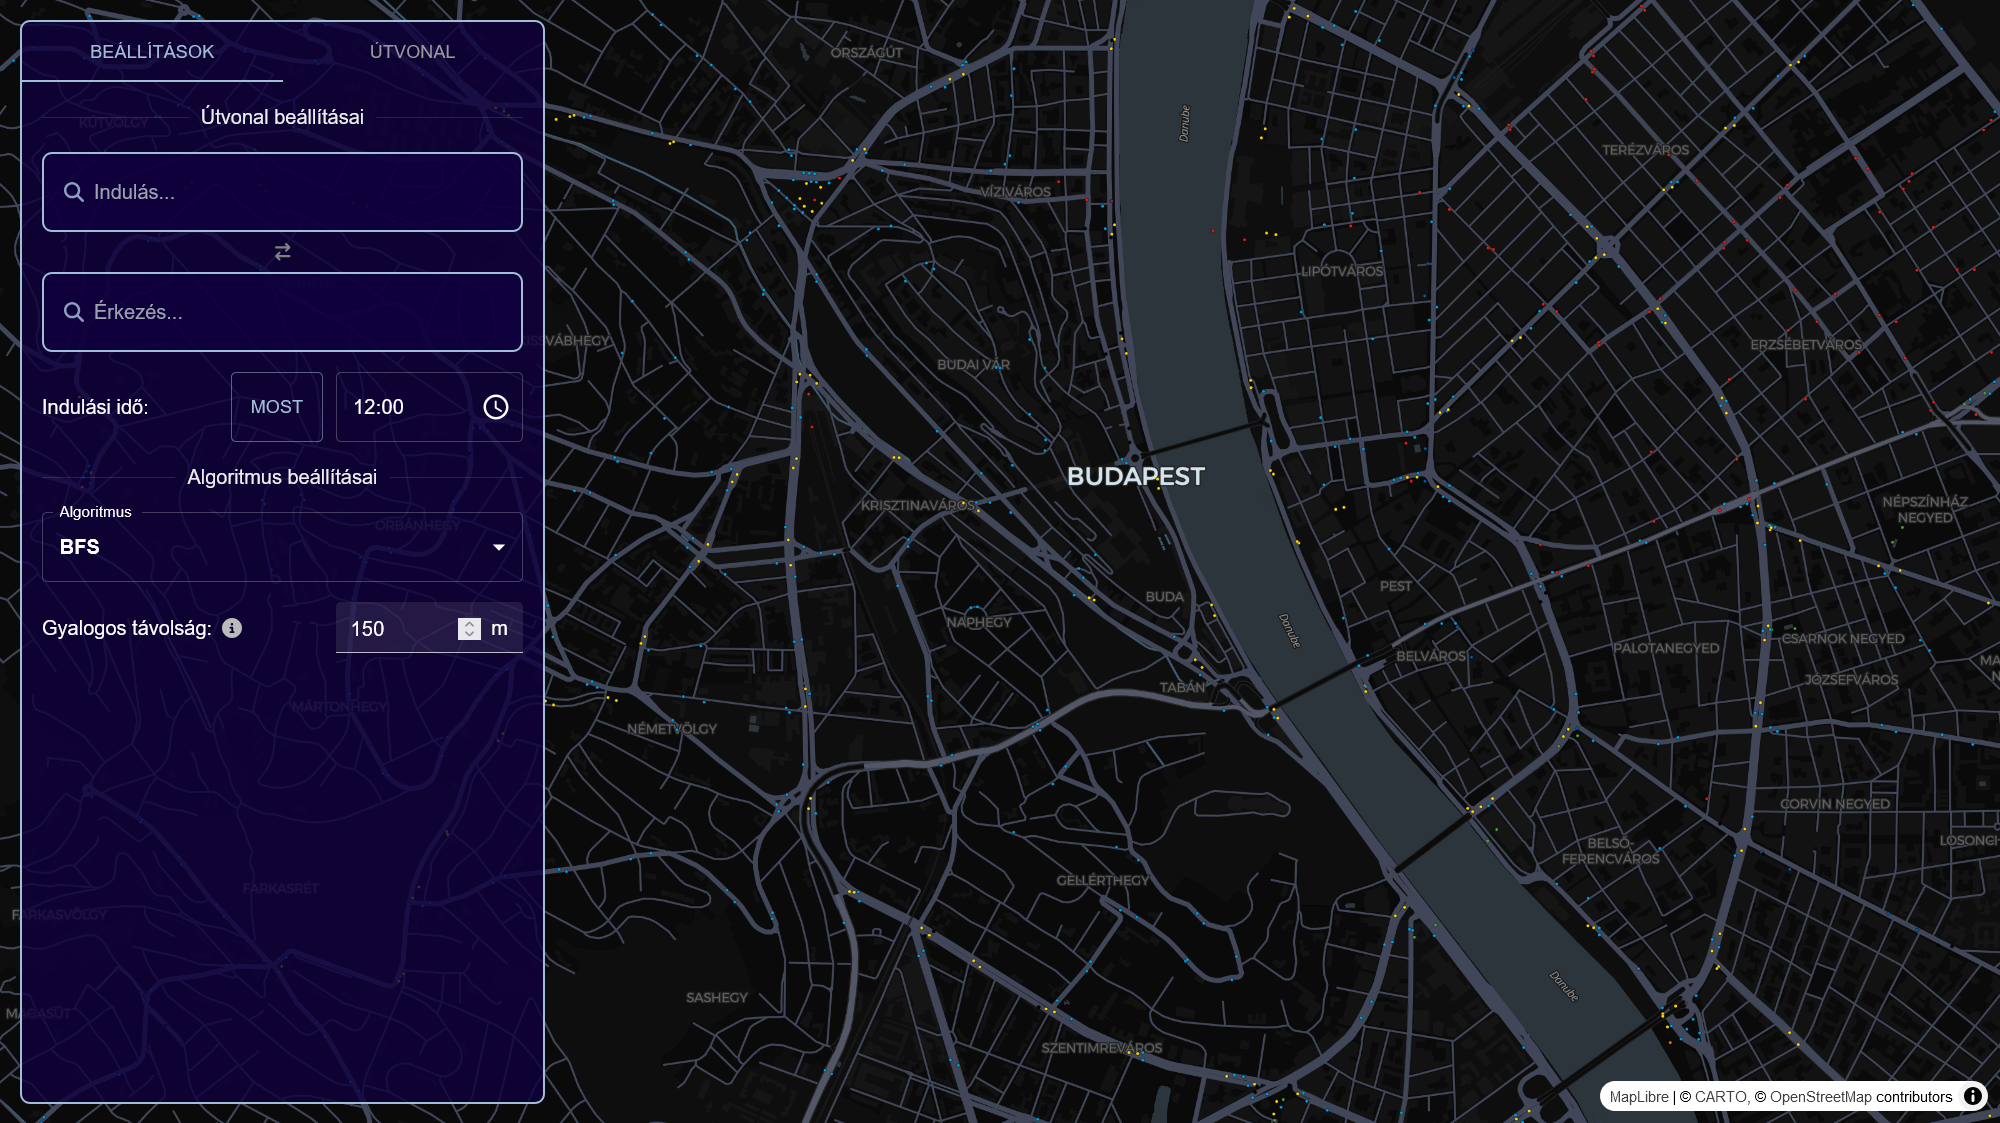
\includegraphics[width=0.8\textwidth]{screenshot_welcome}
	\caption{Az alkalmazás felülete térképpel és vezérlőpanellel}
	\label{fig:screenshot-welcome}
\end{figure}

A térkép navigációja egérrel történik; a térkép nagyítása és kicsinyítése a görgetőkerékkel, a térkép mozgatása pedig az egér bal gombjának lenyomásával és húzásával. A térképen a BKK és a MÁV-HÉV járatainak a megállói láthatók, amik egy-egy színes körrel van jelölve, melyeknek a színét a megállóhoz tartozó járatok színe\footnote{A színek a közlekedési társaságok által használt, közismert színek (pl. a villamosok sárgák, a trolik pirosak).} határozza meg.

\section{Definíciók}

\begin{itemize}
	\item \textbf{Gráf:} Formálisan csúcsok és élek halmaza, ahol minden él két csúcsot köt össze. Az alkalmazás által használt modellben a közlekedési hálózatot egy irányított, súlyozott gráffal modellezzük, így "gráf" alatt a továbbiakban ezt értjük, amennyiben mást nem jelzünk.
	\item \textbf{Csúcs:} A gráf eleme, mely egy megállót jelképez. A továbbiakban a "csúcs" és a "megálló" kifejezések egymás szinonimájaként értendőek, kontextustól függően használjuk őket. A csúcsokhoz egyedi azonosítók tartoznak, melyek a forrásadatokból származnak, és az azonos nevű megállókat megkülönböztetését segíthetik elő.
	\item \textbf{Él:} A gráf eleme, mely két csúcsot köt össze. Az élek irányítottak, azaz csak egy irányba utazhatóak; illetve súlyozottak, azaz minden élhez egy súlyt rendelünk, mely az élen való áthaladás költségét jelképezi. Az alkalmazásban két féle él található:
	\begin{compactenum}
		\item \textbf{Utazási él:} Két megálló közötti közvetlen járatot jelképez, melynek a súlya az utazás időtartamának és a járatra való várakozás idejének az összege. Ez utóbbi alól az első utazási él mentesül, hiszen az csak későbbi indulást jelent, nem várakozást.\\\textit{Megjegyzés: A program csak olyan járatokat vesz figyelembe, melyekre a várakozási idő nem haladja meg a 60 percet.}
		\item \textbf{Átszállási él:} Két megálló közötti gyaloglást jelképez, melynek a súlya a $1 \text{perc} + 1 \frac{\text{másodperc}}{\text{méter}}$ képlet alapján számolódik, vagyis minden átszállás alapsúlya 1 perc, ehhez adódik annyi másodperc, amennyi méter az utak közötti távolság légvonalban.\\\textit{Megjegyzés: Amennyiben az útvonal első éle átszállási él, annak 0 a súlya --- ez azért van, mert könnyű az azonos nevű és egy helyen lévő megállókat összekeverni választáskor, és ezzel a módszerrel akadályozza meg a program azt, hogy egy ilyen hiba miatt hosszabbnak tűnjön az út, mint amilyen valójában.}
	\end{compactenum}
\end{itemize}

\section{Útvonal beállításai}

Útvonal tervezéséhez szükség van egy indulási időpont\footnote{Az indulási idő budapesti időzóna szerint értendő, az alapértelmezett értéke az aktuális helyi idő.}, illetve egy kiinduló- és egy úticél megadására. Célpontoknak a térképen szereplő megállók közül kell választani, egyéb koordináta/cím megadása nem lehetséges. Ezeknek a megadására a vezérlőpanel "BEÁLLÍTÁSOK" fülén van lehetőség (\ref{fig:screenshot-settings-route}).

\begin{figure}[H]
	\centering
	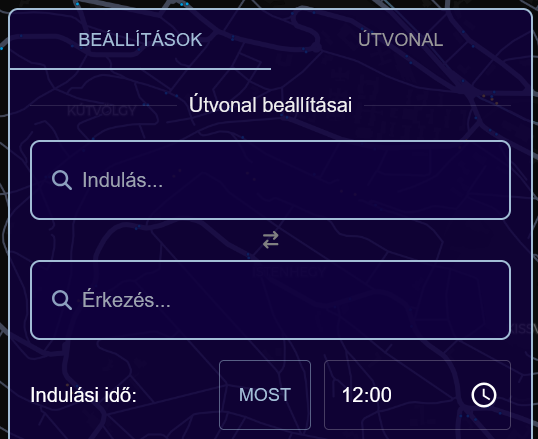
\includegraphics[width=0.5\textwidth]{screenshot_settings_route}
	\caption{Az indulási idő, illetve a kiinduló- és célállomás beállítása}
	\label{fig:screenshot-settings-route}
\end{figure}

Állomások választásához a megfelelő mezőbe kell írni, majd kattintással kiválasztani a megfelelő megállót --- nem elég a nevét beírni, hiszen több, egymástól távoli megálló is rendelkezhet ugyanazzal a névvel (\ref{fig:screenshot-search-stop}). Megfelelő megálló választásához segítségképpen a listában a megállókból induló járatok is megjelennek az adott megálló neve alatt.

A kiinduló- és célállomás felcserélése a két beviteli mező közti dupla nyílra kattintva lehetséges (\ref{fig:screenshot-settings-route}).

\begin{figure}[H]
	\centering
	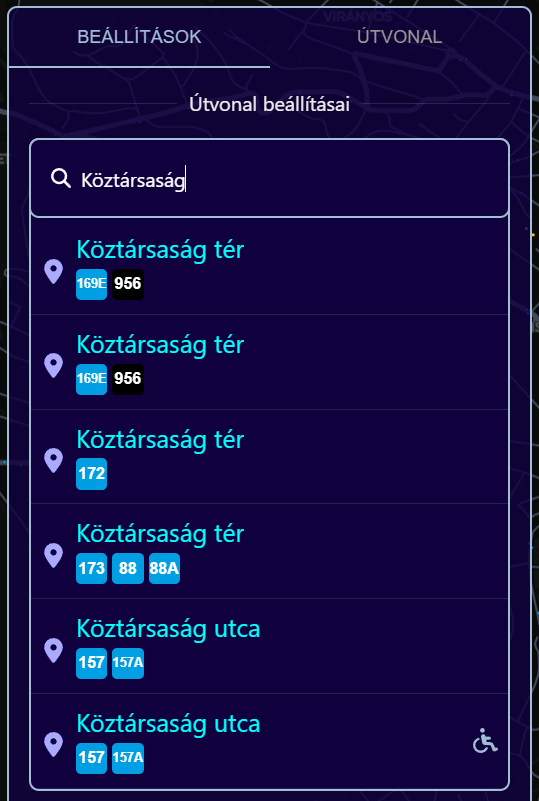
\includegraphics[width=0.4\textwidth]{screenshot_search_stop}
	\caption{Az egyik \emph{Köztársaság tér} nevű megálló Törökbálinton, a másik Pécelen található}
	\label{fig:screenshot-search-stop}
\end{figure}

A térképen az egeret egy megálló fölé helyezve megjelenik annak a neve (\ref{fig:screenshot-tooltip-stop-name}); ez segítséget nyújthat, ha nem ismerjük a célpontunk közelében lévő megállók nevét.

\begin{figure}[H]
	\centering
	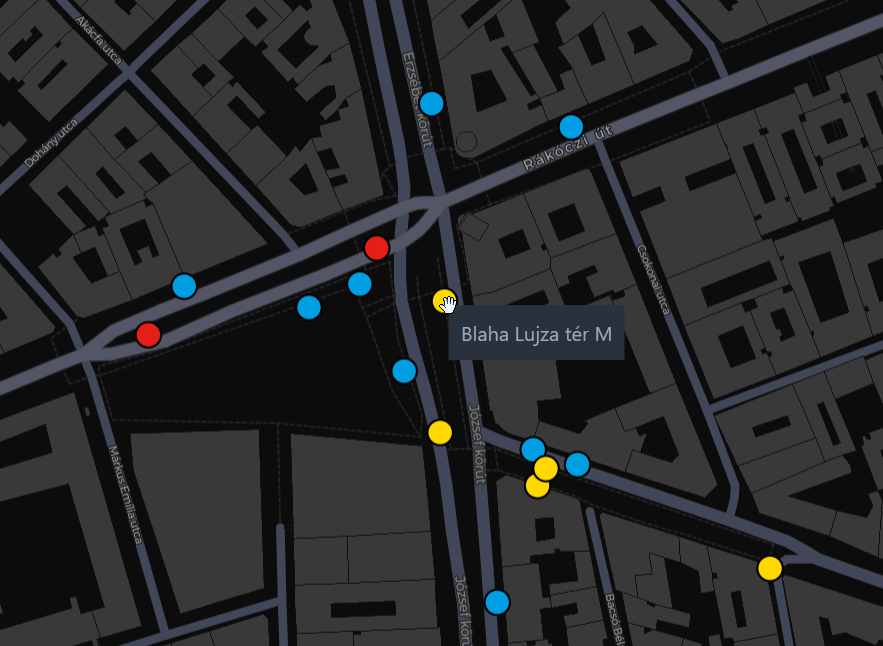
\includegraphics[width=0.8\textwidth]{screenshot_tooltip_stop_name}
	\caption{A kurzor alatt lévő megálló neve egy információs buborékban jelenik meg}
	\label{fig:screenshot-tooltip-stop-name}
\end{figure}

\section{Algoritmus kiválasztása}

\subsection{Választható algoritmusok}

Az útvonalkereséshez négy különböző algoritmus használható, ezekről részletesebben a \ref{ch:algo}.~fejezetben olvashatunk.

\paragraph{Áttekintés az algoritmusokról:}
\begin{enumerate}
	\item \textbf{BFS}: A "Breadth-First Search", azaz szélességi gráfbejárás egy soralapú algoritmus, ahol az újonnan felfedezett megállók egy sor (FIFO adatszerkezet) végére kerülnek be, így először az 1 megálló távolságra lévő megállók kerülnek felfedezésre, majd a 2, stb. . Az algoritmus alapvetően súlyozatlan gráfokon operál, súlyozott gráfokra való alkalmazásakor is figyelmen kívül hagyja az élek súlyát. Ennek következtében az útkeresés eredményeként garantáltan a legkevesebb megállóból álló utat kapjuk meg, attól függetlenül, hogy az adott út mennyi időbe telik. Ennek az algoritmusnak a futásideje egy hagyományos gráfon a legrosszabb esetben $O(|V| + |E|)$, ahol $V$ a csúcsok, $E$ az élek száma a gráfban.
	\item \textbf{Dijkstra-algoritmus}: Az algoritmus a feltalálójáról, Edsger W. Dijkstra informatikusról kapta a nevét, és egy súlyozott gráfban keresi meg a legkisebb súlyú utat egy kiindulópontból az összes többi csúcsba. Az algoritmus a BFS-sel szemben egy prioritási sort használ, ahol a sor elemei a gráf csúcsai, és súly szerinti sorrendben kerülnek feldolgozásra. (Egy-egy csúcs súlya jelen esetben a kezdőállomásból való utazási távolságnak felel meg.) Az alkalmazásban elérhető algoritmusok közül ez az egyetlen, amely garantálja a legrövidebb utazási időt, viszont futásidőben a prioritási sor manipulálásának a komplexitásának\footnote{Az alkalmazás egy kupaccal implementálja a prioritási sort, így egy elem beillesztésének és eltávolításának a komplexitása legrosszabb esetben egyaránt $O(\log n)$.} következtében az algoritmus komplexitása is magasabb a BFS-hez képest. Az algoritmus futásideje egy hagyományos gráfon a legrosszabb esetben $O((|V| + |E|) \log |V|)$.
	\item \textbf{Mohó algoritmus}: A mohó algoritmus a Dijkstra-algoritmushoz hasonlóan egy prioritásos soron alapul, azonban bevezeti a heurisztika fogalmát. A heurisztika egy olyan függvény, amely egy "megérzést" ad egy adott csúcsról, azaz megbecsüli, hogy az adott csúcs mennyire jó választás lehet a következő lépésben. Ebben az alkalmazásban ennek az implementációja a csúcs távolsága a célállomástól, a Föld felszínén egyenes vonalban utazott méterekben mérve\footnote{A képlet ugyan nem veszi figyelembe a tengerszint feletti magasságot, de ez Budapesten és környékén nem tesz drasztikus különbséget, így elfogadjuk közelítésnek.}. Az algoritmus a prioritási sorban a heurisztika értéke szerinti sorrendben dolgozza fel a csúcsokat, így általában sokkal gyorsabban eljut a célállomásba, viszont a BFS-hez hasonlóan ez sem veszi figyelembe az utazási időt, így praktikus használatra általában nem alkalmas. Az algoritmus futásideje egy hagyományos gráfon a legrosszabb esetben $O((|V| + |E|) \log |V|)$.
	\item \textbf{A* algoritmus}: Az A* algoritmus egy továbbfejlesztett mohó algoritmus, amely a Dijkstra-algoritmus és a mohó algoritmus előnyeit igyekszik ötvözni. Az algoritmus a csúcsok súlyát (azaz a kezdőállomástól való utazási időt) és a heurisztikát (a csúcs távolságát a célállomástól) együtt veszi figyelembe a prioritási sorban, így a legjobb választásnak tűnő csúcsokat feldolgozva igyekszik a lehető leggyorsabban eljutni a célállomásba. A* algoritmus választásakor módunk van megadni egy súlyozó faktort, amellyel a heurisztika értékét szorozzuk, így az algoritmus viselkedését befolyásolhatjuk. Alacsonyabb szorzó esetén a Dijkstra-algoritmusra hasonlító viselkedést kapunk (lassabb futásidő, de rövidebb út), magasabb szorzó esetén a mohó algoritmushoz hasnlót (gyorsabb futásidő, de könnyebben eltér a legrövidebb úttól). Az alapértelmezett szorzó $1$, de saját tapasztalataim szerint a $0.3-0.5$ körüli súly jó egyensúlyt biztosít a futásidő és a "használható" eredmény között. Az algoritmus futásideje egy hagyományos gráfon a legrosszabb esetben $O((|V| + |E|) \log |V|)$.
\end{enumerate}

\paragraph{Röviden összefoglalva:}

\begin{compactitem}
	\item \textbf{BFS:} Legkevesebb megállóból álló útvonalat ad, de nem veszi figyelembe az utazási időt.
	\item \textbf{Dijkstra:} Garantáltan a legrövidebb utazási időt adja, de magasabb futásidővel jár.
	\item \textbf{Mohó:} Általában jelentősen gyorsabb a futásideje, de sem az utazási időt, sem az utazott megállók számát nem veszi figyelembe.
	\item \textbf{A*:} Kompromisszum a Dijkstra és a mohó algoritmus között, súlyozó faktorral befolyásolhatjuk a viselkedését.
\end{compactitem}

\subsection{Algoritmusok beállításai}

Az alapértelmezett algoritmus a BFS. Ezt az útvonal beállításai alatt, úgyszintén a vezérlőpanel "BEÁLLÍTÁSOK" fülén lehet megváltoztatni (\ref{fig:screenshot-settings-algorithm}).

\begin{figure}[H]
	\centering
	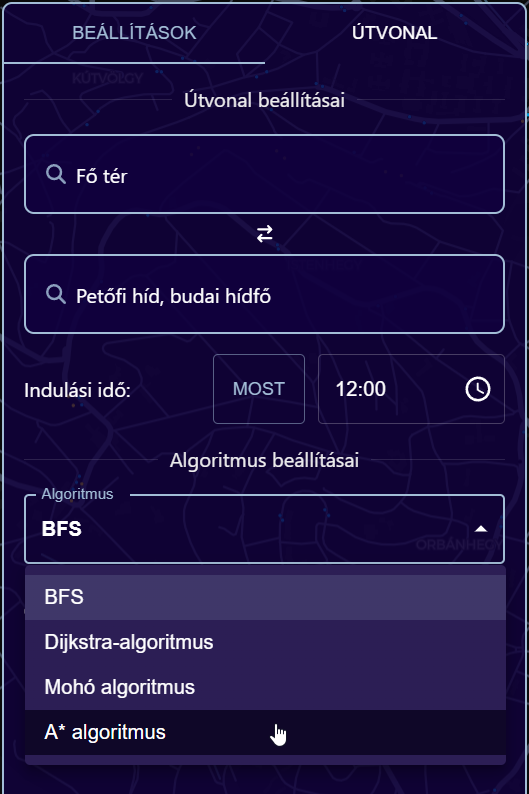
\includegraphics[width=0.5\textwidth]{screenshot_settings_algorithm}
	\caption{Az elérhető algoritmusok listája}
	\label{fig:screenshot-settings-algorithm}
\end{figure}

Választott algoritmustól függetlenül beállítható az is, hogy mi a maximális sétáló távolság, amin belül az alkalmazás felajánl átszállásokat. Ennek az alapértelmezett értéke 150 méter, ami tapasztalataim szerint általában elég azonos nevű, egy csoportban lévő megállók közti átszálláshoz.

Amennyiben a választott algoritmus az A*, akkor a heurisztika súlyozó faktora is beállítható, mely alapértelmezetten $1$ (\ref{fig:screenshot-settings-heuristic}).

\begin{figure}[H]
	\centering
	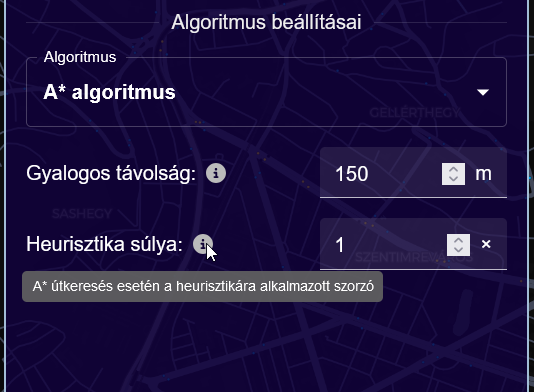
\includegraphics[width=0.7\textwidth]{screenshot_settings_heuristic}
	\caption{A beállításokat információs buborékok magyarázzák}
	\label{fig:screenshot-settings-heuristic}
\end{figure}

\section{Útvonal tervezése}

Amennyiben megtörtént a kezdő- és célállomás megadása, illetve az algoritmust és annak paraméter(ei)t is beállítottuk, megkezdődhet az útvonal tervezése. Ez a vezérlőpanel "ÚTVONAL" fülén történik, mely érvényes beállítások megadása után válik kattinthatóvá (\ref{fig:screenshot-route-initial}).

\begin{figure}[H]
	\centering
	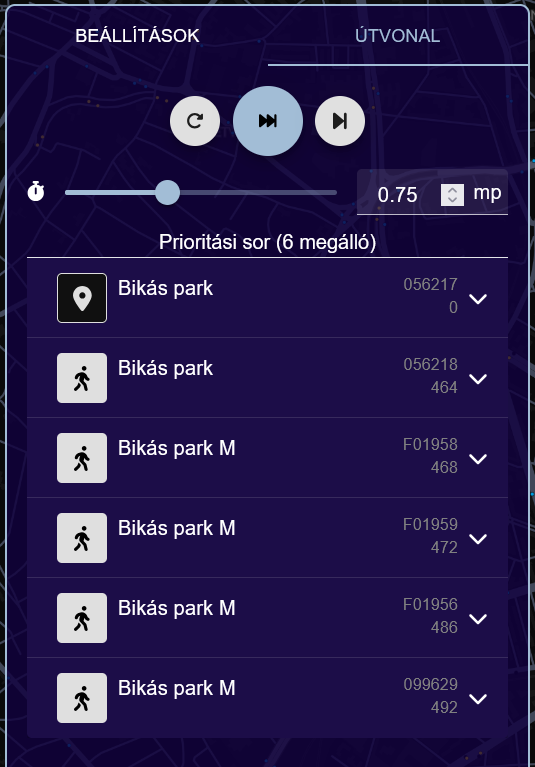
\includegraphics[width=0.4\textwidth]{screenshot_route_initial}
	\caption{Az algoritmus alapállapota az "ÚTVONAL" fülön}
	\label{fig:screenshot-route-initial}
\end{figure}

\subsection{Az algoritmus futtatása}

A fül tetején az algoritmus léptetésére szolgáló gombok találhatók, melyek a következők:
\begin{itemize}
	\item \textbf{Újraindítás}: Az algoritmus visszaállítása a kezdőállapotba.
	\item \textbf{Futtatás}: Az algoritmus addig fut, amíg el nem éri a célállomást. Amíg az algoritmus fut, a többi gomb nem érhető el, ez pedig átváltozik \textbf{Szüneteltetés} gombbá, ami leállítja az algoritmust.
	\item \textbf{Léptetés}: Az algoritmus egy lépéssel halad előre, majd megáll.
\end{itemize}

Ezek alatt egy csúszka található, amelyen azt állíthatjuk be, hogy az algoritmus léptetéskor mennyit várakozik két lépés között. Az alapértelmezett értéke $0.75$ másodperc.
\textit{Megjegyzés: Természetesen lehetséges, hogy egy csúcs feldolgozása tovább tart a várakozási időnél, különösen alacsony értékek esetén.}

\subsection{Az algoritmus állapota}

Amíg az algoritmus nem talált utat a célállomásba, addig a fent említett irányítógombok alatt láthatóak azok a megállók (és olyan sorrendben), amiket az algoritmus következőként fog feldolgozni. A megállók melletti ikon(ok) jelzik, hogy az adott megállóhoz milyen úton érkeztünk. Indulóállomás ez az ikon egy sötét háttéren lévő helyjelző pont, átszállási él esetén egy gyalogló ember, utazási él esetén pedig a járat ikonja és száma látható (\ref{fig:screenshot-icons}).

\begin{figure}[H]
	\centering
	\subcaptionbox{Indulóállomás ikonja}{
		
\includegraphics[scale=2]{screenshot_icon_source}}
	\hspace{5pt}
	\subcaptionbox{Átszállási él ikonja}{
		
\includegraphics[scale=2]{screenshot_icon_walking}}
	\hspace{5pt}
	\subcaptionbox{Utazási él ikonjai}{
		
\includegraphics[scale=2]{screenshot_icon_tram}}
	\caption{A megállók ikonjai azt jelzik, hogy milyen úton érkeztünk az adott csúcsba}
	\label{fig:screenshot-icons}
\end{figure}

Egy-egy megállóra kattintva lenyílik egy további részleteket tartalmazó információs doboz, melyben az adott megállóhoz való érkezés ideje, az odáig megtett út ideje, a csúcs heurisztikája (távolsága a célállomástól méterben), az útban lévő utazási élek száma, illetve a csúcs súlya látható (\ref{fig:screenshot-route-card}). Ez utóbbi az algoritmustól függően van a fentiek alapján kiszámítva.

Ezeken az információkon kívül a dobozban a megállóig tartó út is látható, mely a megállók neveit, azonoítóját és az utazás módját jelölő ikonokat tartalmazza.

\begin{figure}[H]
	\centering
	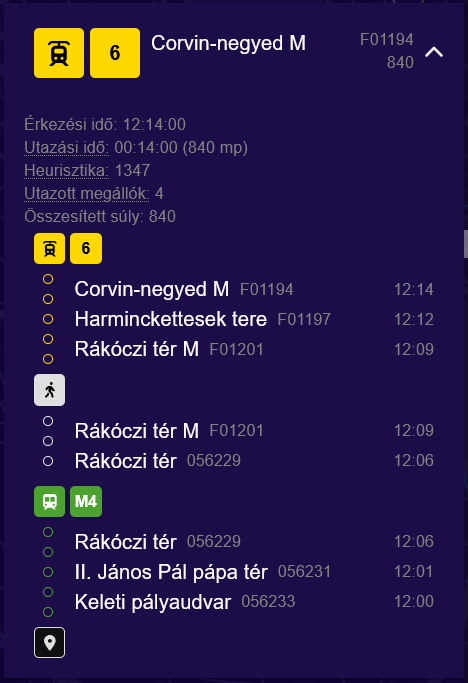
\includegraphics[width=0.5\textwidth]{screenshot_route_card}
	\caption{A megálló részletes információi}
	\label{fig:screenshot-route-card}
\end{figure}

Ezen ismeretek birtokában nincs más hátra, mint lépésről lépésre végignézni az algoritmus futását, és megfigyelni, hogy milyen útvonalon jutunk el a célállomásig.

\subsection{Útvonalak a térképen}

Az algoritmus futása közben a térképen is ki vannak rajzolva a sorra következő megállók, illetve az a kiindulóállomásból vezető út. Az út a megfelelő közlekedési eszköz színével, illetve gyalogos él esetén szürkével (és egy egyenes vonallal) van jelölve. Az egeret egy utazási él fölé helyezve megjelenik annak a járat neve és az utazás hossza is (\ref{fig:screenshot-route-map-started}).

\begin{figure}[H]
	\centering
	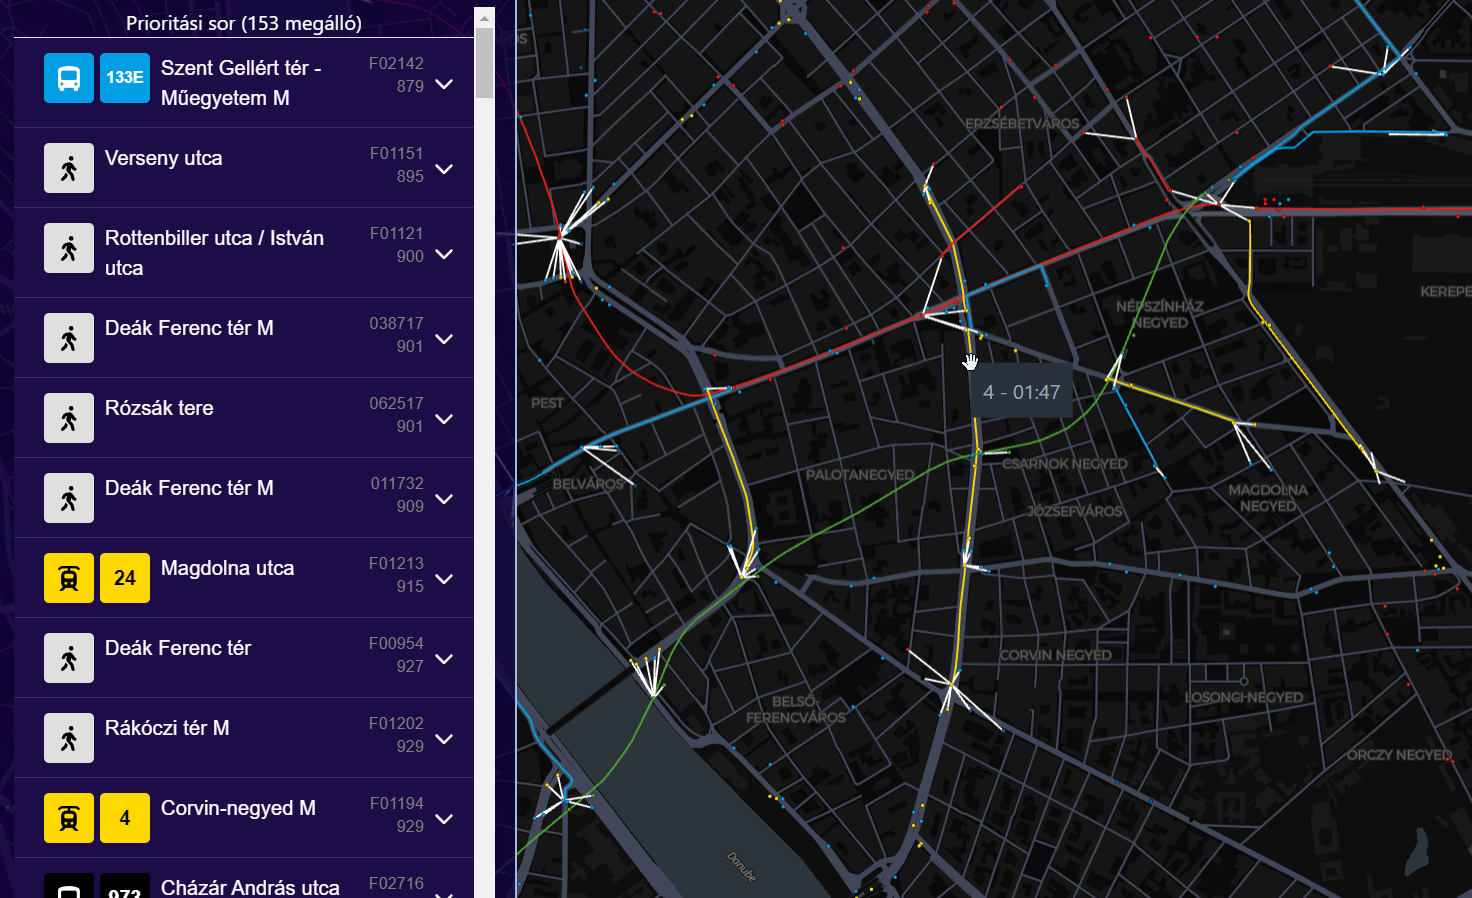
\includegraphics[width=1\textwidth]{screenshot_route_map_started}
	\caption{Az utazás hossza egy megálló távolságra értendő}
	\label{fig:screenshot-route-map-started}
\end{figure}

Amennyiben az algoritmus megtalálta a célállomást, a térképen csak az az út marad megjelenítve, és az oldalsó menüben is az út megállóinak a listája lesz látható (\ref{fig:screenshot-route-map-finished}).

\begin{figure}[H]
	\centering
	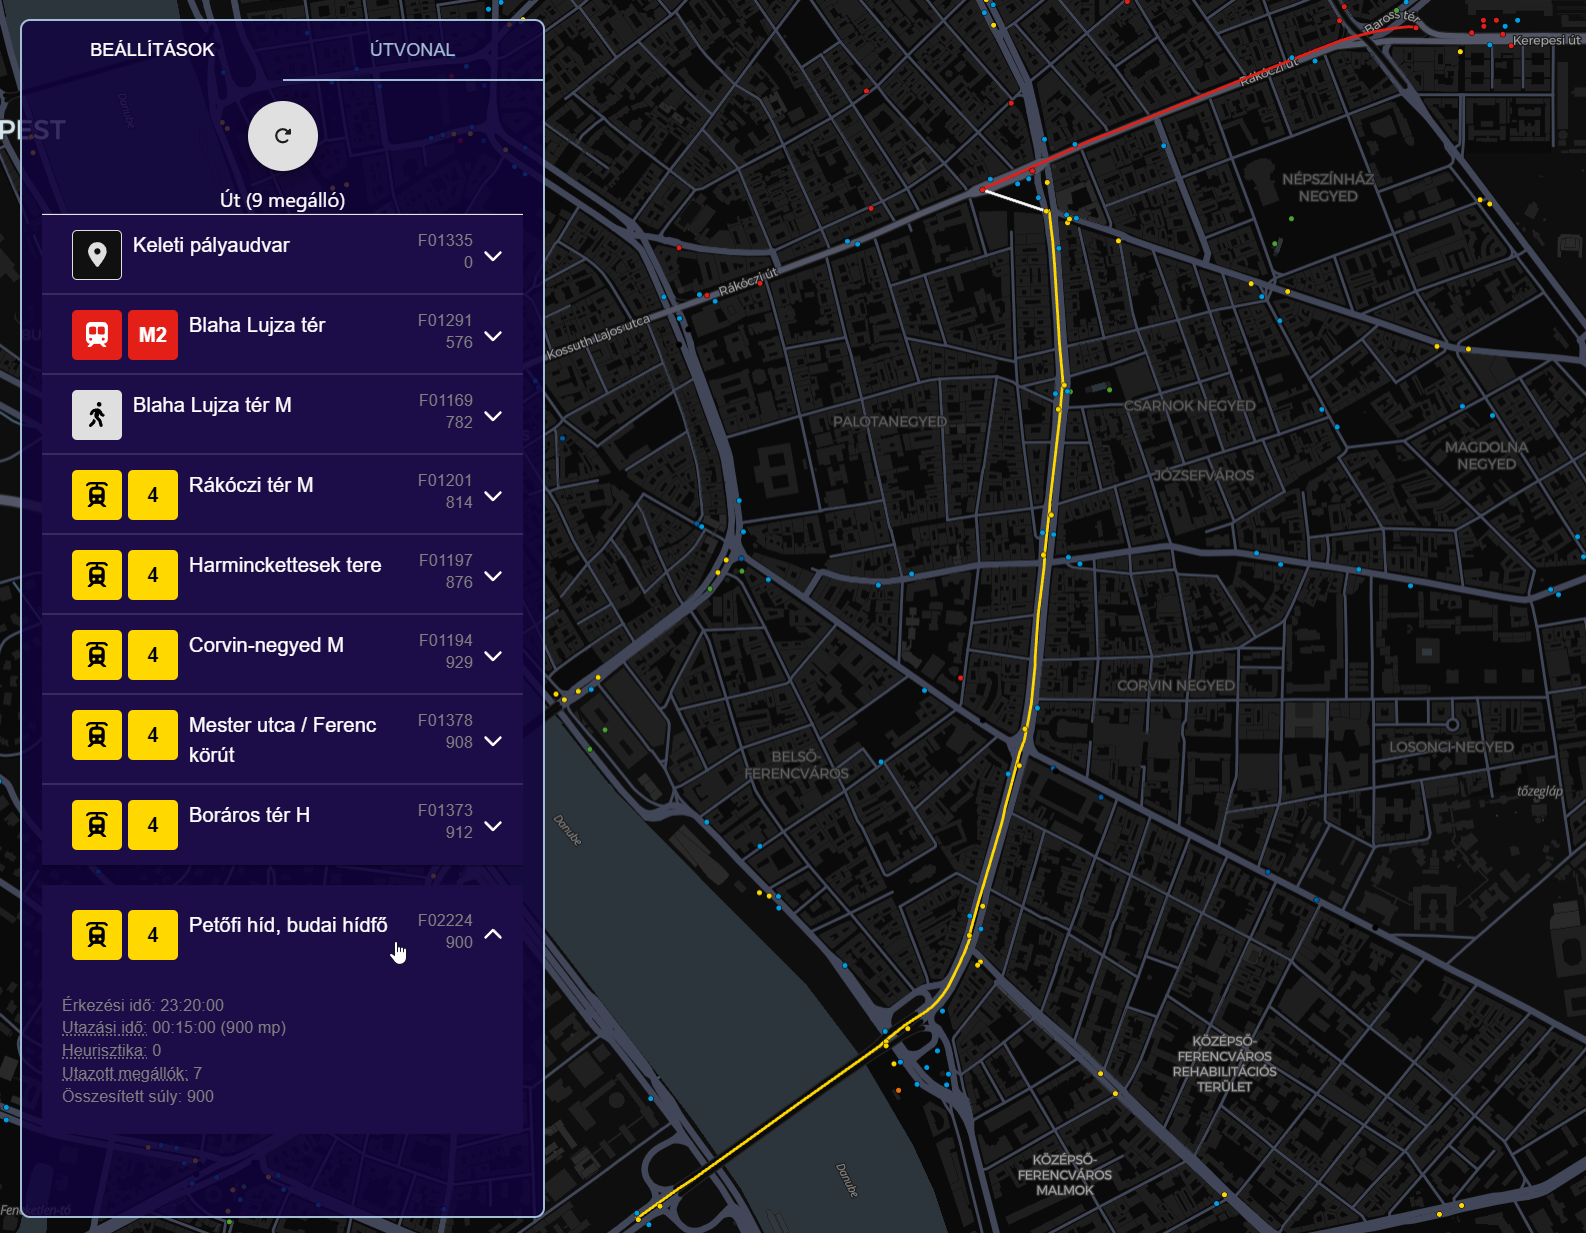
\includegraphics[width=1\textwidth]{screenshot_route_map_finished}
	\caption{Kész útvonal a térképen}
	\label{fig:screenshot-route-map-finished}
\end{figure}

\subsection{Megjegyzés az átszállásokról}

Ugyan a hétköznapokban általában "egy megállóként" szokás gondolni az egymás mellett lévő, azonos nevű megállókra, a valóságban nem ilyen egyszerű a helyzet. A forrásadatban a fizikai megállók külön-külön vannak azonosítva, így a program számára akár két olyan megálló is teljesen különállónak tűnhet, ami a valóságban ugyanahhoz a vonalhoz tartozik, csak az egyiknél a járat az egyik irányban, a másiknál az ellentétes irányban áll meg. Ennek következtében, ha pusztán tömegközlekedéssel keresnénk utat, akkor az alkalmazás nem javasolna olyan átszállásokat, ahol két járat egymás mellett lévő megállói között kellene átszállni; még a célállomást is eltévesztené, amikor az út rossz oldalára érkezik.

Erre természetes megoldás a gyalogos élek bevezetése, így az egymás közelében lévő megállókat szinte egy megállóként kezelhetjük. A program ezt úgy valósítja meg, hogy amint egy új utazási élt ismer meg, a célpontjától sétatávolságra lévő megállókat is hozzáadja az ismert megállók listájához, átszállási éllel összekötve őket az eredeti megállóval. Ugyanígy viselkedik egy útvonaltervezés megkezdésekor, amikor az indulóállomás közelében lévő megállókat "fedezi fel".

Ennek mellékhatásaként amennyiben a választott úticélunkhoz el lehet jutni közvetlen oda érkező járattal is, és egy korábban felfedezhető (pl. Dijksra-algoritmus esetén egy 1 perccel hamarabb elérhető) megállóból való sétálással is, akkor a program a sétálást tartalmazó utat fogja megtalálni, akkor is, ha a sétálás 1 percnél tovább tartana. Ez egy apró, de említésre érdemes bökkenő, hiszen a Dijkstra-algoritmustól azt várnánk, hogy minden esetben a leggyorsabb utat találja meg a két végpont között.

